\documentclass[titlepage,a4paper]{article}

\usepackage{a4wide}
\usepackage[colorlinks=true,linkcolor=black,urlcolor=blue,bookmarksopen=true]{hyperref}
\usepackage{bookmark}
\usepackage{fancyhdr}
\usepackage[spanish]{babel}
\usepackage[utf8]{inputenc}
\usepackage[T1]{fontenc}
\usepackage{graphicx}
\usepackage{float}
\usepackage{fancyvrb}

\pagestyle{fancy} % Encabezado y pie de página
\fancyhf{}
\fancyhead[L]{TP1 Smalltalk - Federico del Mazo}
\fancyhead[R]{Algoritmos y Programación III - FIUBA}
\renewcommand{\headrulewidth}{0.4pt}
\fancyfoot[C]{\thepage}
\renewcommand{\footrulewidth}{0.4pt}

\begin{document}
\begin{titlepage} % Carátula
	\hfill
\includegraphics[width=6cm]{logofiuba.jpg}
    \centering
    \vfill
    \Huge \textbf{Trabajo Práctico 1 — Smalltalk}
    \vskip2cm
    \Large [7507/9502] Algoritmos y Programación III\\
    Curso 1 \\ % Curso 1 para el de la tarde y 2 para el de la noche
    Segundo cuatrimestre de 2017 
    \vfill
    \begin{tabular}{ | l | l | } % Datos del alumno
      \hline
      Alumno: & del Mazo, Federico \\ \hline
      Número de padrón: & 100029 \\ \hline
      Email: & federicodelmazo@hotmail.com \\ \hline
  	\end{tabular}
    \vfill
    \vfill
\end{titlepage}

\tableofcontents % Índice general
\newpage

\section{Introducción}\label{sec:intro}
El presente informe reúne la documentación de la solución del primer trabajo práctico de la materia Algoritmos y Programación III que consiste en desarrollar una aplicación de un sistema de comercio electrónico en Pharo utilizando los conceptos del paradigma de la orientación a objetos vistos hasta ahora en el curso.

\section{Supuestos}\label{sec:supuestos}
% Deberá contener explicaciones de cada uno de los supuestos que el alumno haya tenido que adoptar a partir de situaciones que no estén contempladas en la especificación.

El mayor supuesto encontrado es a la hora de modificar el precio de una compra. ¿Cuál es la mejor forma de modelar que una compra pueda ser modificada por distintos conceptos? Pensarlo de manera que solo funcione para una compra con envío o una compra con garantía termina pareciendo una forma muy cerrada de plantearlo. En cambio, la solución propuesta es una clase nueva dedicada específicamente a estas 'especialidades' en las compras, la clase \textbf{Adicional}. Sea un cupón de descuento o un cobro de envío, la idea es crear una forma genérica de que la compra pueda acceder a distintos adicionales, que sean intercambiables y combinables, y pueda aplicarlos todos sobre su propio precio. De esta forma, si mañana se quisiese, por ejemplo, agregar funcionalidad a ''Anticipo'', ''Pago en cuotas'' u otros, podría hacerse sin tener que indagar en la clase Compra, ya que ahora hay una clase dedicada específicamente a ello.

\section{Modelo de dominio}\label{sec:modelo}
% Explicación concisa del diseño general del trabajo.

\begin{description}
\item[AlgoBay] La clase principal del trabajo modela un mercado y tiene como responsabilidad ser la intermediaria entre todo objeto presente. Si se crea un producto, una compra, un cupón o demás, estos tienen que pasar por esta clase. De esta forma, se tiene un registro de cuanto cuesta cada producto, en que compra están situados, y no tenerlos a todos estos trabajando independientemente sin moderador.
\item[Producto] Los productos son los bienes que van a ser comprados por las compras, dentro de los mercados.
\item[Compra] Ya con un mercado creado con productos dentro, todo bien que yo vaya a comprar tiene que ser situado en el objeto compra para poder finalizar la transacción
\item[Adicional] Siempre que una compra tenga un modificador especial que le cambie el precio, sea para aumentar o disminuir, tendrá un adicional. Actualmente hay implementados 3 adicionales como subclases de esta clase abstracta:
\subitem Envío: El cobro por envío de las compras adiciona un valor a la compra
\subitem Garantía: El cobro de una garantía adicionará un porcentaje de la compra a esta
\subitem Cupón: Un cupón de descuento disminuirá en un porcentaje de la compra cuanto es el valor de esta misma
\end{description}

\section{Diagramas de clase}\label{sec:diagramasdeclase}
% Uno o varios diagramas de clases mostrando las relaciones estáticas entre las clases.  Puede agregarse todo el texto necesario para aclarar y explicar su diseño. Recuerden que la idea de todo el documento es que quede documentado y entendible cómo está implementada la solución.

Para el diagrama de clase muestro como todo pasa por la clase AlgoBay. Crear una compra es en contexto de un mercado, crear un producto y agregarlo a la compra también. Por otro lado tenemos las tres clases que heredan de Adicional, abstracta, que son agregados a la clase Compra, según lo requiera AlgoBay a la hora de crearla.

\begin{figure}[H]
\centering
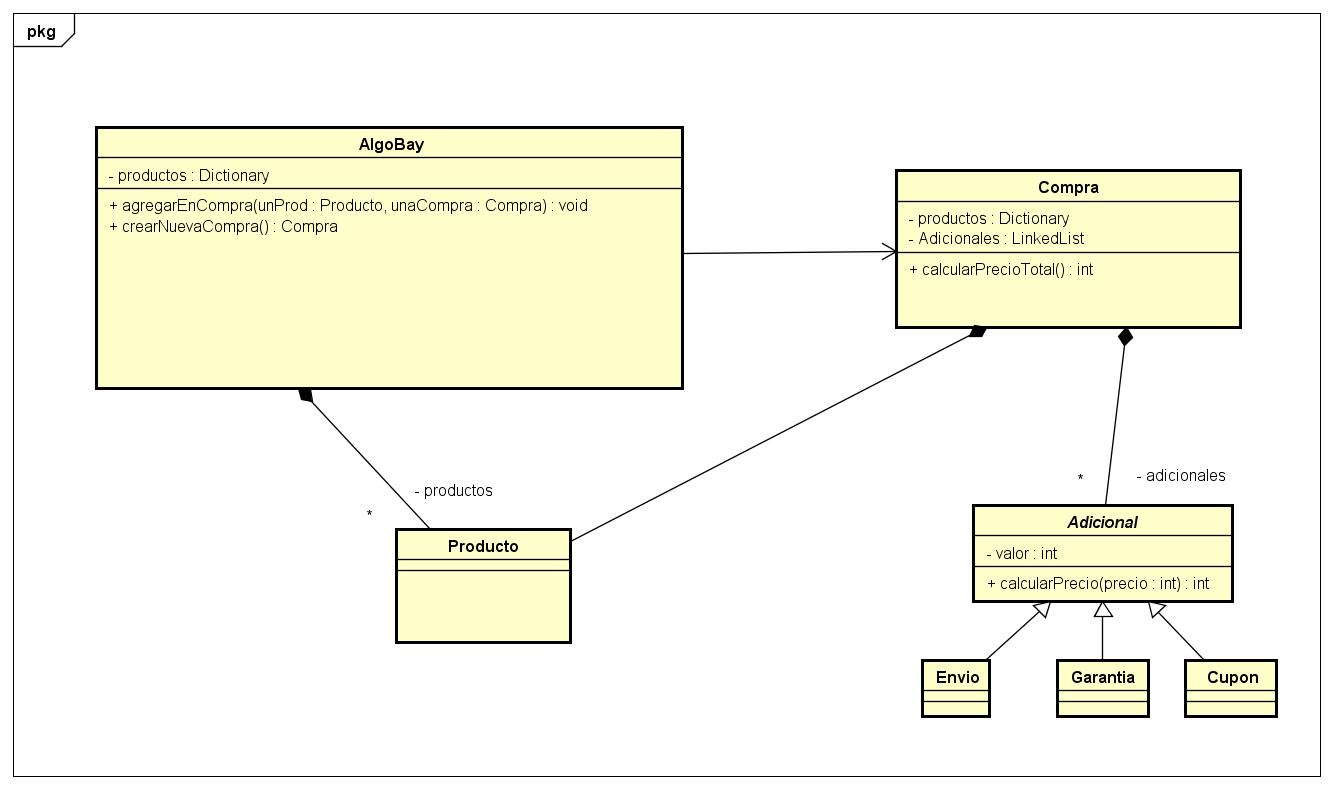
\includegraphics[width=1\textwidth]{0clases.jpg} 
\caption{\label{fig:class01}Diagrama conciso del programa.}
\end{figure}

\section{Detalles de implementación}\label{sec:implementacion}
% Explicaciones sobre la implementación interna de algunas clases que consideren que puedan llegar a resultar interesantes.

\subsection{AlgoBay}
Surgió una cuestión de cómo implementar la idea de que no haya cupones de descuento acumulables. El problema surge en que hay que asumir de quien es la responsabilidad de decidir cual es el cupón vigente. Sea del mercado, de la compra, o del mismo cupón, de alguna forma hay que encargarse de que no se pisen dos cupones en simultaneo. La solución propuesta para esto fue que el mercado, AlgoBay, sea el encargado de que cada vez que agregue un cupón a una compra, retire el presente y compare cual es el vigente de los dos, en este caso, el más grande. Luego, simplemente adiciona el cupón a la compra. De esta forma, la compra misma no es la encargada de recibir dos cupones e inestablemente elegir el mejor para ella, sino que solamente recibe las ordenes de arriba.

\begin{verbatim}
AlgoBay>>> agregarCupon: enCompra:
|cupon_actual mejor_cupon|
cupon_actual := unaCompra retirarCupon.
mejor_cupon:= unaCompra elegirMejorCupon: cupon_actual y: unCupon.
unaCompra agregarAdicional: mejor_cupon
\end{verbatim}

Un segundo supuesto planteado es en el de los valores iniciales de los objetos creados por las pruebas, en este caso, envíos y garantías. En el contexto del trabajo, la garantía es siempre del 10\% y el envío es siempre de \$100. La implementación propone que al momento de crear cada adicional, en AlgoBay, se permita seleccionar el valor para este objeto, de manera que no este dentro del código del adicional, pero si del mercado, y de esta forma solo tenga que modificarse la creación de este y no el código base. Para concluir con esta implementación, se agregaron las excepciones correspondientes a poner valores no permitidos.


\subsection{Compra}
El mayor problema en la clase \textbf{Compra} fue el cálculo de los precios, teniendo en cuenta los adicionales de la compra. La decisión tomada fue la de armar una lista (\textbf{LinkedList}) de los adicionales de la compra, y por un lado tener el método \textbf{calcularPrecioBruto} y el resultado de este ser el que utilice \textbf{calcularPrecioTotal} iterando sobre la lista de adicionales.

\begin{verbatim}
Compra >>> calcularPrecioBruto
|sumatoria|
sumatoria := 0.
productos valuesDo: [:producto | sumatoria:=sumatoria + (producto getPrecio)].
^ sumatoria
\end{verbatim}


\begin{verbatim}
Compra >>> calcularPrecioTotal
|precio|
precio:= self calcularPrecioBruto.
adicionales do: [:atributo | precio:= atributo calcularPrecio: precio].
^ precio.
\end{verbatim}

\subsection{Adicional}
Lo complejo de la clase adicional fue como hacer que cada subclase pueda responder al mismo mensaje, el aplicado por compra, de manera distinta. Por lo tanto, se aplicó polimorfismo con herencia, donde todas las clases hijas heredan el método \textbf{calcularPrecio} de la clase abstracta \textit{Adicional} pero cada una la aplica de manera distinta.

\vspace{1\baselineskip}
\noindent
\begin{minipage}{0.5\textwidth}
\begin{Verbatim}

Envio >>> calcularPrecio
|precio_act|
precio_act:=unPrecio.
(precio_act<5000) ifTrue:
	[precio_act:=precio_act+valor].
^ precio_act
\end{Verbatim}
\end{minipage}
\hspace{1\baselineskip}
\begin{minipage}{0.5\textwidth}
\begin{Verbatim}
Garantia >>> calcularPrecio
^unPrecio * (valor/100) + unPrecio

Cupon >>> calcularPrecio
^ unPrecio - (unPrecio*(valor/100)). 
\end{Verbatim}
\end{minipage}\hfill
\vspace{1\baselineskip}

Lo mismo sucede con el atributo \textbf{Valor} de la clase, ya que tiene que haber distintas implementaciones para el mismo llamado desde \textbf{Compra}.
\subitem En un \textbf{Envío} el valor es un número positivo para adicionar directamente
\subitem En una \textbf{Garantía} el valor es un porcentaje a sumarle al precio
\subitem En un \textbf{Cupón} el valor es un porcentaje a descontar.

\section{Excepciones}\label{sec:excepciones}
% Explicación de cada una de las excepciones creadas y con qué fin fueron creadas.

\begin{description}
\item[AlgoBayProductoNoPresente] Teniendo el método \textbf{getProducto} para obtener un producto del mercado, si este no es encontrado, se lanzará esta excepción.
\item[ProductoPrecioNegativoError] Al agregar un producto al mercado, si este intenta ser agregado con un precio negativo, saltara esta excepción, ya que esto rompe el modelo planteado.
\item[AdicionalPorcentajeInvalidoError] Sea a la hora de crear un cupón de descuento, o de crear una garantía, si el valor no es un porcentaje valido, saltará esta excepción.
\item[AdicionalEnvioNegativoError] Siendo que en el modelo vigente siempre se cobra de más por un envío, y nunca se descuenta, si se intenta crear un envío negativo se lanza esta excepción.
\end{description}

\section{Diagramas de secuencia}\label{sec:diagramasdesecuencia}
% Mostrar las secuencias interesantes que hayan implementado. Pueden agregar texto para explicar si algo no queda claro.

El primer diagrama de secuencia representa lo que pasa cuando se agregan productos al mercado, mostrando la interacción entre \textbf{AlgoBay} y \textbf{Producto}.
\begin{figure}[H]
\centering
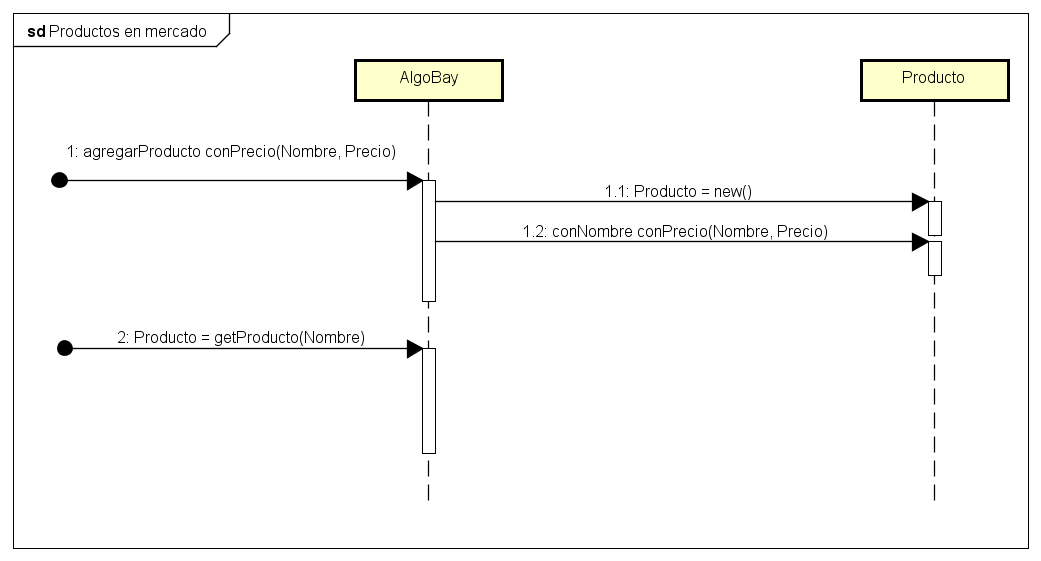
\includegraphics[width=0.9\textwidth]{1productos.png}
\caption{\label{fig:seq01}Agregar un producto al mercado.}
\end{figure}

En el segundo se ve como se crea una compra simple, sin adicionales, y se pide el precio total de esta.
\begin{figure}[H]
\centering
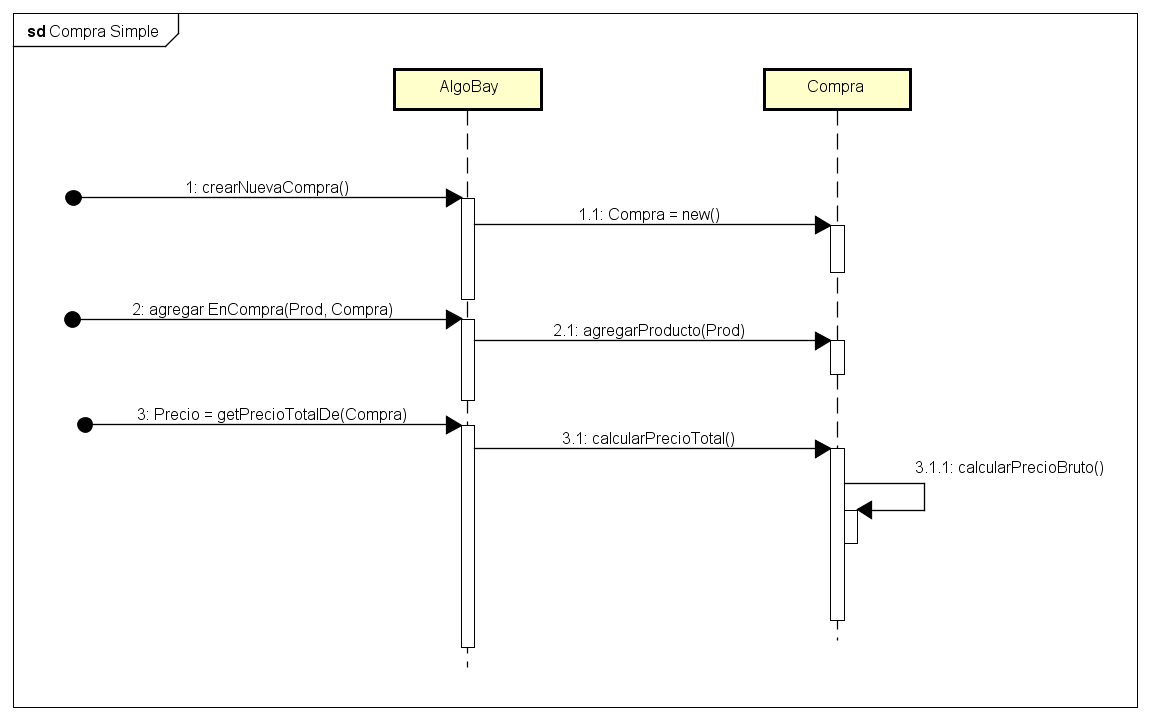
\includegraphics[width=1\textwidth]{2compra.png} 
\caption{\label{fig:seq02}Crear una nueva compra, agregar productos y pedir su precio.}
\end{figure}

En el tercer diagrama se muestra como es la creación de una compra con adicionales, usando de ejemplo el adicional \textbf{Envío}.
\begin{figure}[H]
\centering
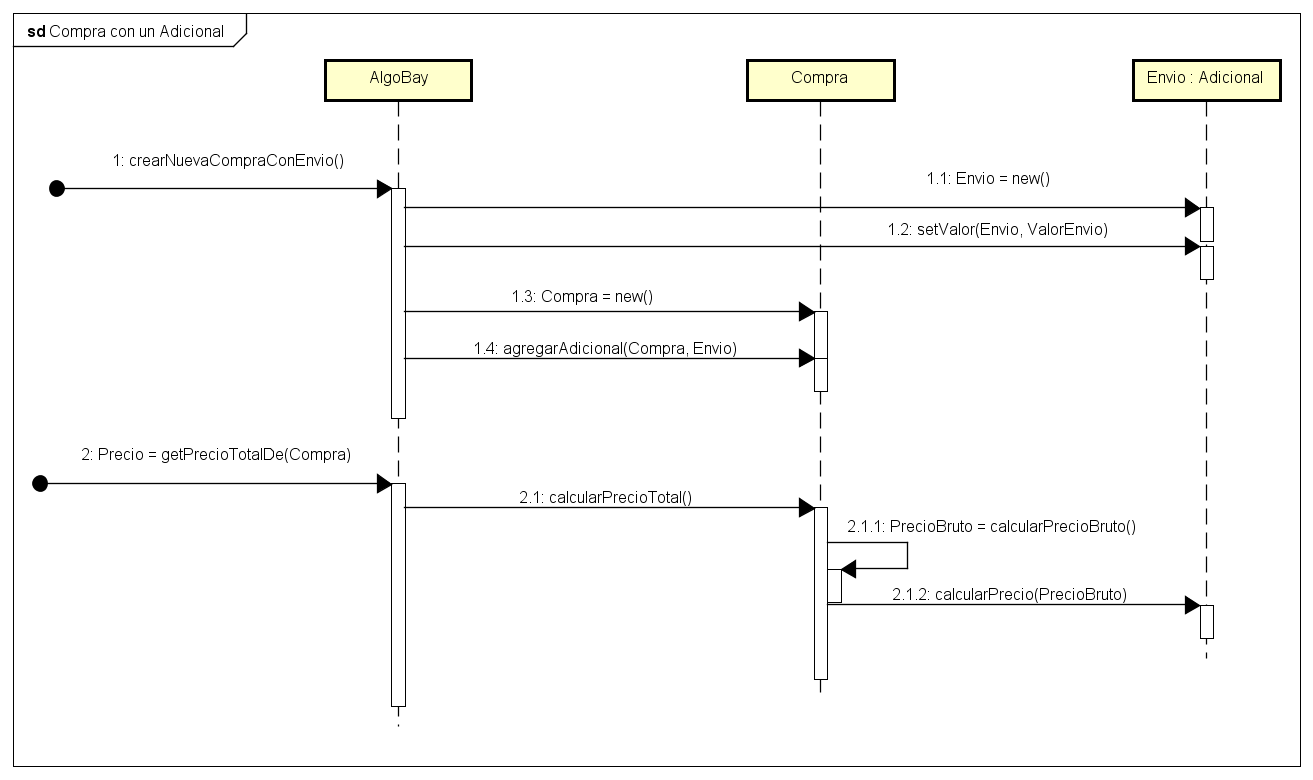
\includegraphics[width=1\textwidth]{3compraenvio.png} 
\caption{\label{fig:seq03}Crear una compra con un adicional.}
\end{figure}

El ultimo diagrama muestra lo sucedido al intentar agregar dos cupones a la misma compra.
\begin{figure}[H]
\centering
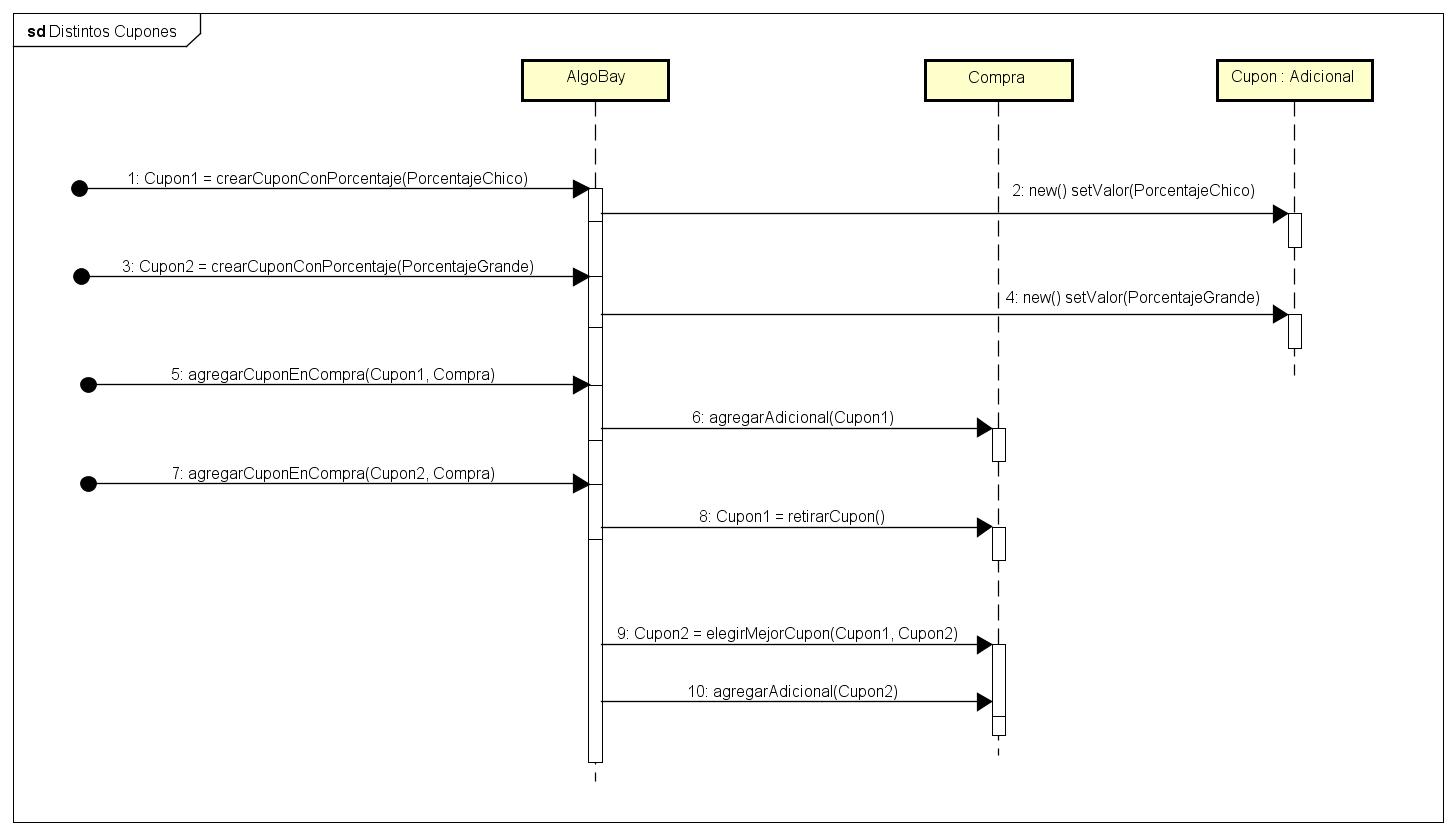
\includegraphics[width=1\textwidth]{4cupones.png} 
\caption{\label{fig:seq04}Manejo de cupones en simultaneo.}
\end{figure}

\end{document}
